\documentclass[a4paper]{article}

\usepackage{mhchem}%化学符号的宏包
\usepackage{cite}%多个文献引用
\usepackage{graphicx}
\usepackage{array}%调节表格行高
\usepackage{multirow,makecell}%多行表格
\usepackage{tabularx}%表格固定列宽
\usepackage{subfigure}
\usepackage{titlesec}%标题格式设置
\usepackage{amsmath}
\usepackage{amssymb}
\usepackage{tabularx}
\usepackage{makecell}
\usepackage{geometry}
\usepackage{float}
\usepackage{setspace}%行距包
\usepackage{siunitx}
\usepackage{mdwlist}
\usepackage{tabu}
\usepackage{enumerate}

\geometry{top=1.54cm,bottom=2.54cm,left=2.5cm,right=2.5cm}


\begin{document}
\begin{center}
\bf\Large
EE 105 Feedback Control Systems\par
Department of Electrical and Computer Engineering\par
Tufts University Fall 2018\par
Homework \#1\par   
\end{center}
\begin{table}[H]
\begin{center}
\begin{tabular*}{\textwidth}{@{\extracolsep{\fill}}lcr}
Name: {\it Shang Wang} &Student ID: {\it 1277417} &E-mail: {\it shang.wang@tufts.edu}\\
\hline
\end{tabular*}
\end{center}
\end{table}

\section{Problem 1: Thermal management of a small satellite}
\begin{enumerate}[(a)]
\item Solve the differential equation pertaining to the “day” side of the orbit to get an equation for the elapsed time needed for the solar flux to heat the satellite from some initial temperature $T_0$ to some warmer temperature $T$. 
\item Solve the differential equation pertaining to the “night” side of the orbit to get an equation for the elapsed time needed for the solar flux to heat the satellite from some initial temperature $T_0$ to some colder temperature $T$.   
\item Using Matlab or your favorite tool,  generate parametric plots showing temperature vs time for each phase of the orbit over a temperature interval from 236.163 K to 243.388 K.   If you use the parameters given on slide 21 from Session 2, you should get heat and cooling time intervals corresponding to a 45-minute half orbit, with a modest temperature excursion of about 7 degrees K.   Think about why the temperature excursions on the moon are so much greater.
\end{enumerate}
{\bf Answer: }\\
(a) Based on physics, we have the differential equation pertaining to the "Day".
\begin{equation}
\pi R^2 F -4\pi R^2\sigma T^4 = mc\frac{{\rm d}T}{{\rm d}t}
\end{equation}
In which, $R$,$m$,$c$ are the radius, mass and specific heat of the satellite respectively, $F$ is solar flux, $\sigma$ is Stefan-Boltzmann constant.\\  
\begin{equation}
A (T_f^4 - T^4) = \frac{{\rm d}T}{{\rm d}t}
\end{equation}
In which $T_f^4 = F/4\sigma$, constant $A = 4\sigma \pi R^2/mc$. Then we seperate the variable $T$ and $t$ into two sides. Then integrate with the initial condition $T(0) = T_0$.
\begin{equation}
\int^t_0 A{\rm d}\tau = \int^T_{T_0} \frac{1}{4T^3_f}\Big(\frac{1}{T_f - T'} -\frac{1}{T_f + T'}+\frac{2T_f}{T^2_f+T'^2}\Big){\rm d}T'
\end{equation}
\begin{equation}
t = \frac{1}{4AT_f^3}\Big(\ln \Big|\frac{T_f+T}{T_f-T}\Big|+2\arctan \frac{T}{T_f}\Big)-t_0
\end{equation}
In which, 
\begin{equation}
t_0 = 	\frac{1}{4AT_f^3}\Big(\ln \Big|\frac{T_f+T_0}{T_f-T_0}\Big|+2\arctan \frac{T_0}{T_f}\Big)
\end{equation}
(b) Differential equation pertaining to the "Night".
\begin{equation}
 -4\pi R^2\sigma T^4 = mc\frac{{\rm d}T}{{\rm d}t}
\end{equation}
Seperate the variables and integrate.
\begin{equation}
	\int_0^t A{\rm d}\tau = \int_{T_0}^{T} \frac{{\rm d}T'}{T^4}
\end{equation}
We have: 
\begin{equation}
	T(t)^3 = 1/\Big(\frac{3\sigma }{mc}\/t+\frac{1}{T_0^3}\Big)
\end{equation}
During both "Day" and "Night", if $t \rightarrow \infty$, the temperature will finally be stable, which means:
$$
\frac{{\rm d}T}{{\rm d}t}\Big|_{t \rightarrow \infty} = 0 
$$ 
So according to Eq(1) and Eq(6), we have: if the satallite stays in the "Day" for long enough, the temperature will finally be $T_f$, while it stays in the "Night" for long, the temperature tends to be zero. \\
\\
(c) Now these are the plots. These plots both start with a "Day" and end with a "Night". Parameters are all from slide 21 from Session 2. The temperature vs time for each phase of the orbit has a interval from 236.163 K to 243.388 K. The gap between "Day" and "Night" is no larger than 7.5K. 
\begin{figure}[hbtp]
\centering
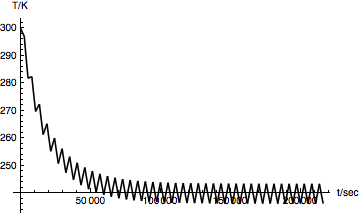
\includegraphics[width=0.5\textwidth]{pic/300decend.png}
\caption{$T_0 = 300$, 40 periods, Temperature(K) vs time(second)} 
\label{300decend}
\end{figure}
\begin{figure}[hbtp]
\centering
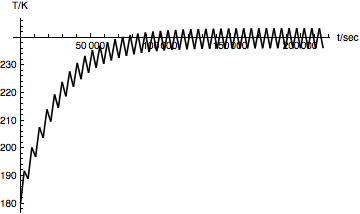
\includegraphics[width=0.5\textwidth]{pic/180ascend.png}
\caption{$T_0 = 180$, 40 periods, Temperature(K) vs time(second)} 
\label{200ascend}
\end{figure}
\section{Problem 2: Ratio}
Complete the exercise at the end of Session 3 by getting an expression for the conversion efficiency of potential energy $kx^2/2$ to kinetic energy $mv^2/2$ in the mass-spring-damper system.
Using Matlab or your favorite tool, plot this as a function of the damping ratio $\zeta$.\\
{\bf Answer: }\\
The solution of the second order differential equation in this problem is :
\begin{equation}
	x(t) = -x_0e^{-\zeta\omega_n t}\Big(\cos(\omega_dt)+\frac{\zeta}{\sqrt{1-\zeta^2}}\sin(\omega_d t)\Big)
\end{equation}
While the spring first reaches its release positon, that is $x(t) = 0$, we have $t = t_0$ and: 
\begin{equation}
	\cos (\omega_d t_0) + \frac{\zeta}{\sqrt{1-\zeta^2}}\sin (\omega_d t_0) = 0
\end{equation}
Assume $\cos(\omega_dt_0) = -\zeta$, which means $\sin(\omega_dt_0) = \sqrt{1-\zeta^2}$ at the same time, which satisfy the condition Eq(10).\\
\begin{equation} 
	v(t) = x'(t) =-x_0\omega_d e^{-\zeta\omega_n t}\Big(-\sin(\omega_dt)+\frac{\zeta}{\sqrt{1-\zeta^2}}\cos(\omega_d t)\Big)+\zeta\omega_n x(t)
\end{equation}
While $x(t_0) = 0$ for the first time, we have:
\begin{equation}
 	v(t_0) = \frac{x_0\omega_d}{\sqrt{1-\zeta^2}}e^{-\zeta\omega_n t_0}
 \end{equation}
Now the ratio $\eta$ becomes:
\begin{equation}
  	\eta = \frac{ mv^2/2}{kx_0^2/2} = \frac{m}{k}\frac{\omega_d^2}{1-\zeta^2}e^{-2\zeta\omega_n t_0}
\end{equation} 
We already know that:
$$
\omega_n = \sqrt{k/m},\ \ \omega_d = \omega_n\sqrt{1-\zeta^2}
$$
So $\eta$ will be: 
\begin{equation}
	\eta = \exp \big[-\frac{2\zeta}{\sqrt{1-\zeta^2}}\arccos(-\zeta)\big]
\end{equation}
Now the plot is:
\begin{figure}[hbtp]
\centering
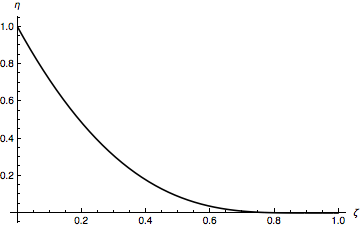
\includegraphics[width=0.5\textwidth]{pic/eta_zeta.png}
\caption{efficiency $\eta$ vs damping ratio $\zeta$} 
\label{eta_zeta}
\end{figure}

\section{Problem 3: Transfer function}
A mass-spring-damper system with an undamped natural frequency $w_n = 1$ can be described with the differential equation:   $F/m = x''+ 2\zeta x' + x$.   Suppose that the system is under steady state sinusoidal forcing,  $F/m=e^{i\omega t}$.  Using Matlab or your favorite tool, generate overlaid log-log plots of the magnitude of the velocity oscillation as a function of excitation frequency w over the range  $0.001< \omega < 1000$,  for values of the damping ratio $\zeta $= 0.01, 0.2, 1.0, and 5.0.
In preparation for class, think about why a low-friction system, whose unforced oscillations last a long time, should be strongly frequency selective for forced oscillations.\\
{\bf Answer: }\\
This is the plot which contains transfer function of  $\zeta = 0.01,\ 0.2,\ 1.0\ \text{and}\ 5.0 $.
\begin{figure}[hbtp]
\centering
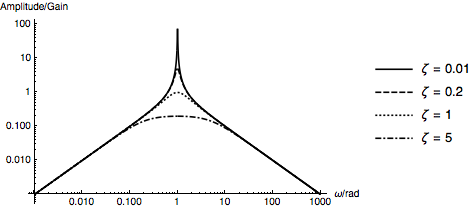
\includegraphics[width=0.6\textwidth]{pic/transfer.png}
\caption{tranfer function of different $\zeta$} 
\label{transfer}
\end{figure}





\end{document}